\documentclass[12pt,a4paper]{article}
\usepackage[brazil]{babel}
\usepackage[utf8]{inputenc}
\usepackage{graphicx}
\usepackage{amsmath}

\usepackage{color}
\definecolor{codegreen}{rgb}{0,0.6,0}
\definecolor{codegray}{rgb}{0.5,0.5,0.5}
\definecolor{codepurple}{rgb}{0.58,0,0.82}
\definecolor{backcolour}{rgb}{0.95,0.95,0.92}

\usepackage{listings}
\lstset{ 
    backgroundcolor=\color{backcolour},   
    commentstyle=\color{codegreen},
    keywordstyle=\color{magenta},
    numberstyle=\tiny\color{codegray},
    stringstyle=\color{codepurple},
    basicstyle=\footnotesize,
    breakatwhitespace=false,         
    breaklines=true,                 
    captionpos=b,                    
    keepspaces=true,                                                  
    showspaces=false,                
    showstringspaces=false,
    showtabs=false,                  
    tabsize=2
}

\title{MEF para Chave de Carro Segura}
\author{Bruno Tatsuya Masunaga Santos\\
        Sistemas Digitais 2018.2}
\date{\today}

\begin{document}
\maketitle

\section{Introdução}
Chaves de Carro precisam ser únicas para cada veículo. Não se espera que outra pessoa, com a chave de um carro do mesmo modelo, consiga desbloquear e entrar no seu carro. Portanto, existem soluções físicas para impedir este tipo de acontecimento. No entanto, as vezes a produção de chaves pode apresentar falhas, de modo que eventualmente alguém consiga entrar num carro que não lhe pertence. Dado este cenário, surge a motivação em desenvolver uma solução digital para este problema, utilizando os conceitos adquiridos na disciplina de Sistemas Digitais, ministrada pelo Prof. Valério Ramos Batista.  

\section{Objetivos}
Deseja-se implementar uma Máquina de Estados Finitos que se baseie num Reconhecedor de Sequência, o qual reconheça o código 1011 em binário, a ser digitado bit a bit pelo usuário. Essa implementação visa abstrair a situação apresentada na Introdução, de modo que para desbloquear um carro seja necessária a emissão do código após a digitação correta da sequência.

\section{Justificativa}
De forma geral, este trabalho representa um projeto de solução segura para resolver os problemas de desbloqueio inesperado de carros e até mesmo outros equipamentos, se o caso se aplica. Sabe-se que, desta forma, possuir uma chave que se encaixe fisicamente não é o suficiente para desbloquear um automóvel. É necessária a digitação de um código, o qual espera-se que apenas o proprietário conheça. Assim, este projeto propõe um aprimoramento da segurança neste quesito.

\section{Metodologia}
Para realizar este projeto, utilizou-se uma modelagem baseada na Máquina de Estados Finitos de Moore. Optou-se por este modelo em detrimento ao modelo de Mealy pelo fato de a Máquina de Moore representar uma solução mais concisa e uma abstração mais adequada para este tipo de problema, na opinião do autor. 

Elaborou-se o Diagrama de Estados Finitos com apenas uma entrada X e uma saída S. A entrada representa um bit da sequência que o usuário digita sucessivamente. A saída representa o desbloqueio do carro: 0 se o carro está bloqueado, 1 se o carro desbloqueia. Este Diagrama foi construído com 5 estados, denominados A, B, C, D e E:
\begin{itemize}
\item O estado A representa a situação inicial do problema, em que não há nenhum bit correto digitado pelo usuário e o carro está bloqueado. Caso o usuário digite o bit 1, então ele vai para o estado B, mas caso digite o bit 0, ele permanecerá no estado A. 
\item O estado B representa a situação onde o sistema reconhece que foi digitado corretamente o primeiro algarismo do código. O carro está bloqueado. Neste caso, se o usuário digitar o bit 0, então ele avançará para o estado C. Caso contrário, ele permanecerá no estado B.
\item O estado C ocorre quando o sistema reconhece corretamente os dois primeiros digitos do código. O carro permanece bloqueado. Se o usuário digitar o bit 1, então o sistema avançará para o estado D. No entanto, se digitar o bit 0, voltará ao estado inicial A.
\item O estado D é atingido quando os três primeiros algarismos do código são digitados corretamente em sequência pelo usuário. O carro ainda está bloqueado. Neste caso, se o usuário digitar o bit 1, então o sistema avança para o estado final E. Caso contrário, ele retornará ao estado C.
\item O estado E é o estado final, e representa a digitação correta da sequência secreta. Agora, o carro é desbloqueado e o sistema emite a saída 1. O carro irá bloquear novamente quando o usuário digitar outro bit. Se digitar 1, então ele retornará ao estado B. Caso contrário, retornará ao estado C.  
\end{itemize}

\begin{figure}[h]
	\centering
	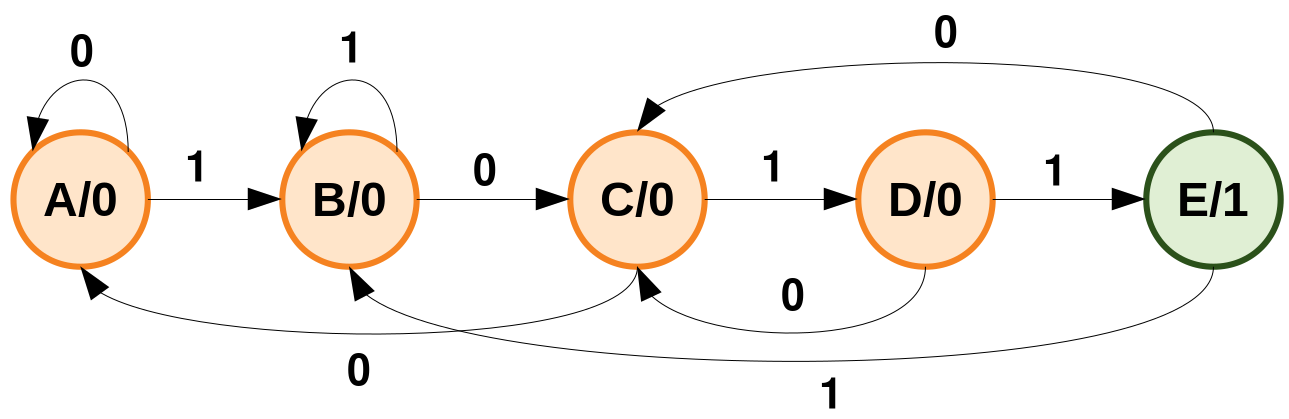
\includegraphics[scale=0.25]{Imagens/diagrama.png}
	\caption{Diagrama de Estados de Moore para o problema}
\end{figure}

A partir do Diagrama, montou-se a Tabela de Estados, que evidencia o fluxo dos estados do sistema:

\begin{table}[h]
\centering
\begin{tabular}{c|c|c|c}
\cline{2-3}
                                     & \multicolumn{2}{c|}{\textbf{Próximo Estado}} &                                     \\ \hline
\multicolumn{1}{|c|}{\textbf{Atual}} & X = 0                  & X = 1               & \multicolumn{1}{c|}{\textbf{Saída S}} \\ \hline
\multicolumn{1}{|c|}{A}              & A                      & B                   & \multicolumn{1}{c|}{0}              \\ \hline
\multicolumn{1}{|c|}{B}              & C                      & B                   & \multicolumn{1}{c|}{0}              \\ \hline
\multicolumn{1}{|c|}{C}              & A                      & D                   & \multicolumn{1}{c|}{0}              \\ \hline
\multicolumn{1}{|c|}{D}              & C                      & E                   & \multicolumn{1}{c|}{0}              \\ \hline
\multicolumn{1}{|c|}{E}              & C                      & B                   & \multicolumn{1}{c|}{1}              \\ \hline
\end{tabular}
\end{table}

Então, utilizou-se o código binário para recodificar os estados, a fim de tornar possível uma representação lógica do sistema. O estado A foi identificado como 000, o B como 001, o C como 010, o D como 011 e o E como 100. Veja a nova tabela abaixo:

\begin{table}[h]
\centering
\begin{tabular}{c|c|c|c}
\cline{2-3}
                                     & \multicolumn{2}{c|}{\textbf{Próximo Estado}} &                                     \\ \hline
\multicolumn{1}{|c|}{\textbf{Atual}} & X = 0                  & X = 1               & \multicolumn{1}{c|}{\textbf{Saída S}} \\ \hline
\multicolumn{1}{|c|}{000}            & 000                    & 001                 & \multicolumn{1}{c|}{0}              \\ \hline
\multicolumn{1}{|c|}{001}            & 010                    & 001                 & \multicolumn{1}{c|}{0}              \\ \hline
\multicolumn{1}{|c|}{010}            & 000                    & 011                 & \multicolumn{1}{c|}{0}              \\ \hline
\multicolumn{1}{|c|}{011}            & 010                    & 100                 & \multicolumn{1}{c|}{0}              \\ \hline
\multicolumn{1}{|c|}{100}            & 010                    & 001                 & \multicolumn{1}{c|}{1}              \\ \hline
\end{tabular}
\end{table}

Desta forma, a partir dessa tabela, obteve-se as equações booleanas para cada digito do código ($D_A$  é o primeiro, $D_B$ é o segundo e $D_C$ é o terceiro) e também para a saída S, utilizando Diagramas de Karnaugh. As imagens abaixo demonstram como esses diagramas foram aplicados:

\pagebreak

\begin{figure}[h]
	\centering
	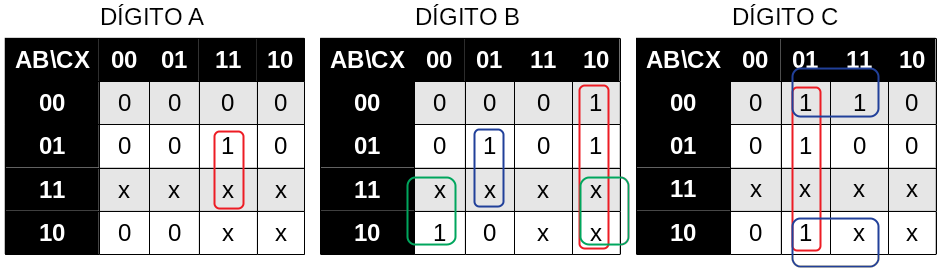
\includegraphics[scale=0.4]{Imagens/karnaughDigits.png}
	\caption{Diagrama de Karnaugh para $D_A$, $D_B$ e $D_C$ do código}
\end{figure}

\begin{figure}[h]
	\centering
	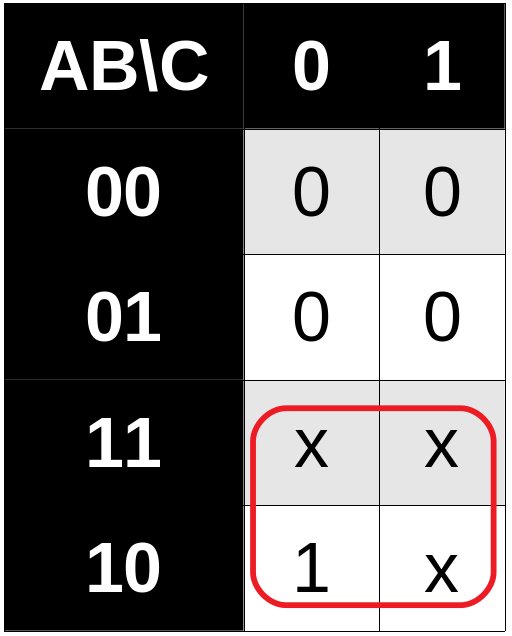
\includegraphics[scale=0.15]{Imagens/karnaughS.png}
	\caption{Diagrama de Karnaugh para a saída S}
\end{figure}


Como é uma Máquina de Moore, a saída depende apenas dos estados. Portanto, o Diagrama de Karnaugh para a saída S foi elaborado sem dependência de X. Assim, obteve-se as seguintes funções booleanas:
\begin{align}
&D_A = BCX \\
&D_B = \overline X(A+C) + B\overline C X \\
&D_C = X(\overline C + \overline B) \\
&S = A
\end{align}

Com tais funções, pôde-se construir o circuito lógico do sistema no software \textbf{Logisim}, que será apresentado na próxima seção. Esse circuito foi elaborado levando em conta uma \textbf{simulação temporal}, de modo que toda dinâmica envolvida funciona com base na subida de um clock. Neste caso, foram utilizados Flip-Flops D para registrar os estados.

Após elaboração do circuito lógico, implementou-se a Tabela de Estados em VHDL. Neste código, construiu-se o funcionamento da transição de estados com base na subida do clock e também uma opção de reset assíncrono do registro (ou seja, retornar ao estado inicial A independente do clock). Além disso, implementou-se a tabela propriamente dita, evidenciando o fluxo dos estados com base nas entradas e a respectiva saída com base nos estados. Essa implementação é mais próxima de uma \textbf{Descrição de Fluxo de Dados} do sistema, já que não implementa os Flip-Flops D e nem mesmo a lógica apresentada no circuito elaborado no Logisim.

Foi elaborado também o Test-Bench com 17 casos de transição de estados (incluindo o uso do reset assíncrono) para o código VHDL elaborado anteriormente, a fim de que ele fosse testado por alguns softwares. Primeiro, fez-se a simulação no \textbf{GHDL} com auxílio do \textbf{GTKWave}. Depois, utilizou-se o \textbf{Quartus II} para elaborar um Test-Bench automático (os testes escolhidos foram os mesmos 17) e o \textbf{ModelSim} para simular o funcionamento do código VHDL elaborado com este Test-Bench. Também foram consultados os visualizadores de RTL e de Technology Map do Quartus II, para verificar o Diagrama Lógico que ele interpreta.

Como o funcionamento do sistema se baseia nos ciclos do clock, o tipo de simulação efetuado nos softwares tem característica temporal, já que a transição dos estados ocorre apenas quando há subida deste clock. Desta forma, são esperados resultados que levam em conta \textbf{atrasos na propagação de sinais}, mesmo que mínimos, em detrimento de um resultado lógico imediato. Todas essas características poderão ser vistas na próxima seção.

\section{Apresentação dos Dados e Análise dos Resultados}
Utilizando o Logisim e as equações booleanas apresentadas anteriormente, obteve-se o seguinte circuito lógico:

\begin{figure}[h]
	\centering
	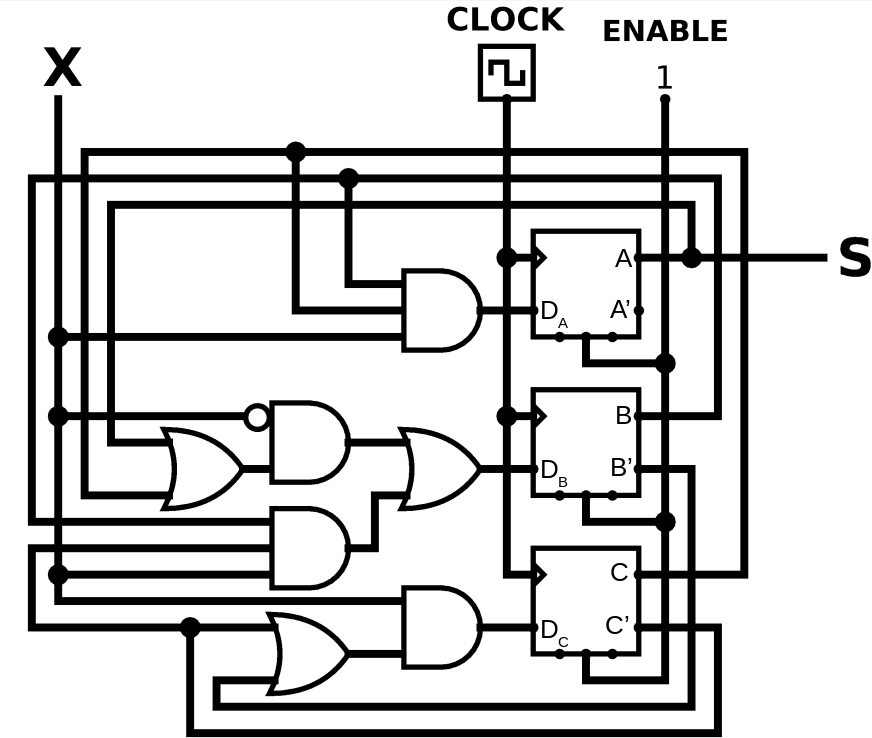
\includegraphics[scale=0.25]{Imagens/logisim.png}
	\caption{Circuito Lógico do sistema elaborado no Logisim}
\end{figure}

Como visto, existe uma lógica de funcionamento que depende do clock. O uso dos Flip-Flops D garantem registro correto do fluxo dos estados.

Agora, a simulação efetuada no GHDL e no GTKWave produziu o seguinte resultado:

\begin{figure}[h]
	\centering
	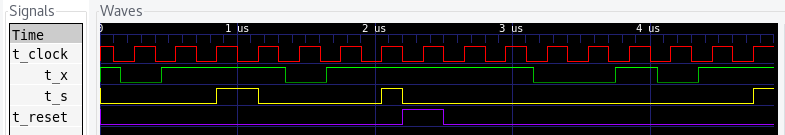
\includegraphics[scale=0.5]{Imagens/gtkwave.png}
	\caption{Simulação do VHDL no GTKWave utilizando o Test-Bench}
\end{figure}

Note que o funcionamento do sistema está correto de acordo com a Tabela de Estados utilizada. A saída S torna-se 1 somente se o código correto (1011) é digitado sequencialmente pela entrada X após quatro ciclos do clock. Veja também o funcionamento do reset assíncrono, que leva o sistema diretamente para o estado A, independentemente do clock. Outro ponto importante é verificar que apesar de as entradas serem digitadas em determinado tempo, o estado do sistema só muda numa subida de clock, demonstrando o caráter temporal da simulação, já discutido anteriormente.

Agora, o carregamento do código VHDL (que não será apresentado no relatório por ser muito grande) no Quartus II produziu os resultados esperados. Primeiramente, os diagramas gerados pelo RTL Viewer e pelo Technology Map podem ser verificados em \textbf{Quartus/Imagens/}. Pelo fato de serem imagens grandes, não serão apresentados no relatório. Agora, a simulação do VHDL no ModelSim produziu o seguinte resultado:

\begin{figure}[h]
	\centering
	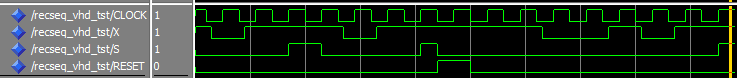
\includegraphics[scale=0.52]{Imagens/modelsim.png}
	\caption{Simulação do VHDL no ModelSim utilizando o Test-Bench gerado pelo Quartus II}
\end{figure}

Veja que o resultado obtido é exatamente o mesmo gerado pela simulação no GHDL e no GTKWave, o que era de fato esperado e, portanto, representa a corretude do código em abstrair a tabela elaborada.

O código VHDL e seu respectivo Test-Bench podem ser verificados em \textbf{VHDL/recSeq.vhd} e \textbf{VHDL/recSeq-tb.vhd}. O Test-Bench gerado pelo Quartus está em \textbf{Quartus/recSeq/simulation/modelsim/recSeq.vht}.

\section{Apresentação de um Exemplo de Funcionamento do Programa}

Todos os resultados obtidos a partir da aplicação da metodologia podem ser reproduzidos. 

Começando pelo circuito lógico, é possível carregá-lo no Logisim a partir do arquivo \textbf{Logisim/circuito.circ}. Para efetuar testes, primeiro habilite o funcionamento do clock, marcando as opções \textsl{Simulate$\rightarrow$Simulation Enabled} e \textsl{Simulate$\rightarrow$Ticks Enabled} no programa. Veja que o clock deverá começar a oscilar. O verde escuro indica o clock em 0 e o verde claro indica o clock em 1. Tente digitar a sequência 1011 no botão da entrada X (basta clicar em cima para mudá-lo). Lembre-se que a passagem do bit digitado em X para os Flip-Flops D se dá somente na subida do clock (na transição do 0 para o 1). O LED da saída S deverá ficar aceso por um ciclo do clock e se apagará na próxima subida.

Para reproduzir a simulação do VHDL no GHDL e GTKWave, abra o terminal no diretório \textbf{VHDL/}. Digite a seguinte sequência de comandos:

\begin{lstlisting}
$ ghdl -a recSeq.vhd
$ ghdl -a recSeq-tb.vhd
$ ghdl -e recSeq-tb
$ ghdl -r recSeq-tb --vcd=simulation.vcd
$ gtkwave simulation.vcd
\end{lstlisting}

Feito isso, insira todos os sinais utilizando a opção \textsl{insert} e utilize o ícone \textsl{Zoom Fit} do programa para ajustar o tempo de simulação para a janela aberta. Com isso, será possível reproduzir a simulação apresentada na seção anterior.

Por fim, para reproduzir todos os testes realizados no Quartus II, basta carregar o diretório do projeto já criado no programa, que se encontra em \textbf{Quartus/recSeq/}. Feito o carregamento, basta seguir as instruções indicadas no tutorial de Quartus disponibilizado para a aula de laboratório da Semana 7 da disciplina de Sistemas Digitais. Os procedimentos realizados no projeto seguiram criteriosamente os passos demonstrados neste tutorial. Desta forma, os resultados obtidos podem ser reproduzidos no RTL Viewer, no Technology Map e no ModelSim.

\section{Conclusão}
Os resultados obtidos demonstraram o funcionamento esperado do modelo proposto nos objetivos. Além disso, os códigos VHDL compilaram e executaram corretamente a partir do GHDL e nas simulações com o Quartus/ModelSim. No entanto, o modelo de Reconhecedor de Sequência aplicado neste modelo não é o ideal para este tipo finalidade. Note que mesmo se o usuário erra o código, os últimos digitos são considerados na próxima avaliação da sequência. Numa situação real, é esperado que o usuário digite os quatro dígitos e o sistema avalie se o código é válido ou não, a partir daí produzindo uma resposta e retornando ao estado inicial. No entanto, este tipo de condição torna-se complexo utilizando as técnicas básicas adquiridas na primeira parte do curso de Sistemas Digitais, de modo que tornaria-se um projeto muito custoso e pouco simples de se desenvolver. Desta forma, considera-se que os objetivos foram atingidos e o projeto foi implementado com sucesso.

\section{Referência Bibliográfica}
Foram consultados apenas os materiais disponibilizados na página da disciplina de Sistemas Digitais no TIDIA. Nenhuma fonte adicional foi utilizada. 

\end{document}